\documentclass[12pt,a4paper]{article}
\usepackage[margin=1in]{geometry}
\usepackage{amsmath,amssymb}
\newcommand{\E}{\mathbb{E}}
\newcommand{\indep}{\perp\!\!\!\perp}
\usepackage{booktabs}
\usepackage{longtable}
\usepackage{graphicx}
\usepackage{tikz}
\usetikzlibrary{arrows.meta, positioning}
\usepackage{float}
\usepackage{needspace}
\usepackage{cite}
\usepackage[colorlinks=true,linkcolor=blue,citecolor=blue,urlcolor=blue]{hyperref}
\hypersetup{pdfborder={0 0 0},breaklinks=true,linktoc=all}
\usepackage{tocloft}
\setlength{\cftbeforesecskip}{3pt}
\setlength{\cftbeforesubsecskip}{1.5pt}
\setlength{\cftaftertoctitleskip}{0.8em}
\renewcommand{\cftsecfont}{\small}
\renewcommand{\cftsubsecfont}{\small}
\setcounter{tocdepth}{2}

\renewcommand{\abstractname}{Abstract}
\makeatletter
\renewenvironment{abstract}{%
  \centerline{\cfttoctitlefont\abstractname}\par\vspace{0.8em}%
  \list{}{%
    \setlength{\leftmargin}{0pt}%
    \setlength{\rightmargin}{0pt}}%
  \item\relax\fontsize{13pt}{15.6pt}\selectfont}
 {\endlist}
\makeatother

\title{From Association to Causation:Multi-Method Propensity Score Analysis of Physical Activity and Cardiovascular Disease with Identification Diagnostics and Mediation}
\author{Liesen Gai \texttt{23307130013@m.fudan.edu.cn}}

\begin{document}

\begin{titlepage}
\centering
\vspace*{2.8cm}
\begingroup
\linespread{1}\selectfont
{\LARGE\bfseries
From Association to Causation:
Multi-Method Propensity Score Analysis
of Physical Activity and Cardiovascular Disease
with Identification Diagnostics and Mediation
\par}
\endgroup
\vspace{2.8cm}
{\Large Liesen Gai\par}
\vspace{0.8cm}
{\large \texttt{23307130013@m.fudan.edu.cn}\par}
\vspace{2.2cm}
\vfill
\end{titlepage}

\newpage
\begin{abstract}
\noindent Under the potential-outcomes framework, this study uses the Ulianova public cardiovascular dataset to estimate the causal effect of physical activity on cardiovascular disease (CVD) risk. Guided by a directed acyclic graph (DAG) and the backdoor criterion, the study specify an adjustment set and triangulate inverse probability weighting (IPW), g-formula, doubly robust augmented IPW (AIPW), propensity score (PS) matching and stratification, and linear probability models (LPM). I systematically assess propensity score overlap (positivity), covariate balance, BMI mediation decomposition, and sensitivity to unmeasured confounding. After controlling for major confounders, physical activity shows a consistent protective association with CVD risk; multiple identification--estimation strategies agree in direction. The protective effect operates mainly through a direct path not mediated by BMI; the mechanism share attributable to BMI is limited. These findings align with international epidemiological consensus that physical activity modifies CVD risk factors and support population-level promotion of regular activity. Because the data are cross-sectional and observational, causal extrapolation requires caution; conclusions should be read as supportive rather than confirmatory evidence.

\vspace{0.6em}
\noindent\textbf{Keywords:} physical activity; cardiovascular disease; causal inference; propensity score; inverse probability weighting
\end{abstract}

\newpage
\tableofcontents

\newpage
\setcounter{page}{1}

\section{Background and Research Questions}

\subsection{Field Context and Prior Evidence}

Globally, insufficient physical activity and sedentary behavior continue to rise and are widely recognized as modifiable risk factors for noncommunicable diseases, especially cardiovascular disease (CVD) \cite{mi2025creview}. Mi et al.\ \cite{mi2025creview}, in a \textit{Circulation Research} review, note that despite decades of accumulating epidemiological evidence and public health guidelines promoting targets such as at least 150 minutes per week of moderate-intensity aerobic activity, large segments of the U.S.\ and global populations still fail to meet recommended activity levels, with disproportionately low activity among racial/ethnic minorities, women, and older adults. Mechanistically, regular physical activity may protect the cardiovascular system by improving endothelial function, reducing systemic inflammation, optimizing blood pressure and lipid profiles, and increasing cardiorespiratory fitness \cite{mi2025creview}. Thus, whether increasing activity lowers CVD risk is a core public health question and a canonical setting for causal inference methods.

Observational studies provide substantial supportive evidence. Garcia et al.\ \cite{garcia2023meta} conducted a dose--response meta-analysis of 94 prospective cohorts with over 30 million participants and found nonlinear inverse associations between non-occupational physical activity and all-cause mortality, CVD mortality, and several cancer outcomes: the largest risk reductions occur from ``inactive'' to roughly 8.75 mMET-hours per week (equivalent to guideline-recommended 150 minutes/week of moderate-to-vigorous aerobic activity). At that dose, the relative risk (RR) of CVD death is approximately 0.71 (95\% CI: 0.66--0.77) and all-cause mortality RR is approximately 0.69; if all insufficiently active individuals reached that level, about 15.7\% of premature deaths could be avoided. Mi et al.\ \cite{mi2025creview} further summarize that higher activity is consistently associated with lower mortality and risk of coronary heart disease, ischemic stroke, heart failure, atrial fibrillation, and other CVD subtypes across age, sex, and baseline health status; pooled analyses of over 2 million participants with questionnaire-assessed activity link meeting guideline activity with roughly 22\% lower mortality, while accelerometer-based studies often report larger effect sizes. Mechanistic literature suggests that activity's impact on CVD is not captured by a single ``total effect'': Chen et al.\ found mediation and moderation through body-fat percentage, blood pressure, and lipids among Chinese adults \cite{chen2023pa}; Wang et al.\ report that moderate-to-vigorous recreational activity partly affects hypertension through obesity indices \cite{wang2023obesity}; Hall et al.\ note that cardiorespiratory fitness (CRF) as a mediator can shift activity-intensity thresholds relevant to cardiometabolic health \cite{bjsports2023crf}. Together, these results portray a landscape of protective associations and multi-pathway mechanisms, providing literature support for the mediation decomposition in this paper.

\subsection{Limitations of Observational Research and Position of This Study}

Moving from association to causation, observational PA--CVD studies face structural limitations that motivate this project. Activity is not randomly assigned: younger, metabolically healthier, and socioeconomically advantaged individuals tend to be more active, and these factors also influence CVD diagnosis, so classical confounding prevents crude comparisons from receiving a causal interpretation \cite{mi2025creview,hernan2024whatif}. In cross-sectional or short-follow-up designs, reverse causation is equally problematic---individuals with existing CVD symptoms or diagnoses may reduce activity, inflating the appearance that active individuals have lower risk \cite{mi2025creview}. When activity is measured by self-report questionnaires or coarse categories, recall bias and misclassification further weaken credibility; Mi et al.\ \cite{mi2025creview} note that questionnaire and accelerometer estimates for the same activity dose can differ severalfold, with varying measurement reliability across devices and populations (e.g., older adults). Even Mendelian randomization (MR) designs do not guarantee robust causal conclusions: Qiu et al.\ \cite{qiu2025mr}, in a two-sample MR study based on European GWAS, found only vigorous physical activity (VPA) showed a modest causal association with major coronary heart disease (IVW OR$=0.95$, 95\% CI: 0.91--0.99), while average activity and other intensity subtypes showed no substantial causal links with eight chronic diseases---suggesting limited genetic instrument representation of ``general activity'' and that MR cannot simply be equated with ``no causal effect of activity on CVD,'' but does show causal evidence strength varies by design. Mi et al.\ \cite{mi2025creview} also emphasize that direct RCT evidence that PA lowers mortality and CVD remains relatively limited; long-term adherence and ethical constraints make large randomized trials difficult. In sum, the field has established a protective direction and dose clues for PA, but on a single observational dataset there remains room for methodological integration and transparent reporting of how to estimate interpretable average causal effects (ACE) under explicit causal assumptions, diagnose identification conditions, decompose mechanisms, and assess residual confounding.

Against this background, I conduct a complete observational causal analysis pipeline using the Ulianova public cardiovascular dataset \cite{ulianova2019kaggle}. Compared with existing literature, I do not claim new biological findings or population-level causal certainty; I focus on a methodologically transparent, reproducible estimation and diagnostic chain under explicit assumptions: under DAG and backdoor guidance, the estimand is $\mathrm{ACE}=\E[Y(1)-Y(0)]$ (risk difference), distinguishing total-effect adjustment from mediation decomposition with respect to BMI \cite{hernan2024whatif,vanderweele2015explanation}; on one dataset I triangulate IPW, g-formula, doubly robust AIPW, linear models, and PS matching/stratification \cite{hernan2024whatif,rosenbaum1983central,robins1994estimation,shahu2023comparison}; I systematically report positivity and covariate balance diagnostics \cite{chen2024iptw}; and under the VanderWeele framework I decompose BMI mediation paths, combining adjustment-set sensitivity, effect modification, and E-value analysis \cite{vanderweele2015explanation,vanderweele2017evalue}. Section~2 states identification assumptions and estimation principles; Section~3 reports multi-method ACE; Sections~4--5 test positivity and balance---only when estimates converge and diagnostics pass do subsequent mechanism and sensitivity discussions become meaningful.

\subsection{Data, Estimand, and Causal Structure}

Data come from the Kaggle Ulianova cardiovascular examination dataset \cite{ulianova2019kaggle} (original file \texttt{cardio\_train.csv} with 70{,}000 records). Before analysis, I exclude 1{,}608 observations with implausible blood pressure ($ap\_hi\in[80,200]$, $ap\_lo\in[40,120]$, and $ap\_hi>ap\_lo$), BMI (15--60), or height (140--220 cm), retaining $N=68{,}392$ valid samples. Note: other small-sample files in the same directory (e.g., UCI Heart Disease) are not used in this study. Outcome $Y$ is CVD diagnosis (prevalence 49.4\%); treatment $A$ is binary self-reported physical activity (80.3\% active). Covariates include age, sex, smoking, alcohol use, cholesterol, glucose, and BMI, matching the multidimensional $L$ structure required for propensity score/IPW methods, with variables measured consistently in the same examination workflow. Importantly, the data are cross-sectional, activity is a coarse self-reported category, intensity and duration cannot be distinguished, objective measurement is unavailable, and reverse causation cannot be ruled out; conclusions should be understood as causal estimation under stated assumptions on this dataset, not a simple replication of Garcia et al.\ \cite{garcia2023meta} or other large prospective meta-analyses.

Under the potential-outcomes framework, let $A_i=1$ denote individual $i$ is physically active, $Y_i=1$ denote CVD presence, and $Y_i(a)$ the potential outcome under treatment $a$. The target estimand is the average causal effect
\[
\mathrm{ACE}=\E[Y_i(1)-Y_i(0)].
\]
If $\mathrm{ACE}<0$, intervening to move the entire population from inactive ($A=0$) to active ($A=1$) would reduce average CVD probability by $|\mathrm{ACE}|$. This differs from an associational comparison of currently active versus inactive individuals, which mixes causal effects with selective entry into activity \cite{hernan2024whatif}.

Figure~\ref{fig:dag} shows the causal structure. Age, sex, smoking, alcohol use, cholesterol, and glucose affect both activity and CVD risk, forming backdoor paths $A\leftarrow L\to Y$; BMI likewise, and may biologically serve partly as mediator $A\to M\to Y$ \cite{wang2023obesity,chen2023pa}. Unmeasured factors $U$ (e.g., family history, diet, healthcare access) that affect both $A$ and $Y$ constitute residual confounding that cannot be directly tested. The primary adjustment set is
\[
L=\{\text{age},\ \text{sex},\ \text{smoking},\ \text{alcohol},\ \text{cholesterol},\ \text{glucose},\ \text{BMI}\},
\]
chosen by the backdoor criterion: after conditioning on $L$, $A$ is conditionally independent of $(Y(1),Y(0))$ \cite{hernan2024whatif,rosenbaum1983central}. The main analysis controls BMI as a confounder to estimate total effect; mechanism analysis later removes BMI from $L$ and treats it separately as mediator $M$ to decompose natural direct effect (NDE) and natural indirect effect (NIE) \cite{vanderweele2015explanation}. The main analysis deliberately does not control concurrent blood pressure: in cross-sectional data, blood pressure may reflect long-term activity effects (mediation) or existing cardiovascular pathology (confounding), and including it risks over-adjusting for mediators or conditioning on colliders \cite{hernan2024whatif}; robustness analysis separately tests adding blood pressure.

\begin{figure}[H]
\centering
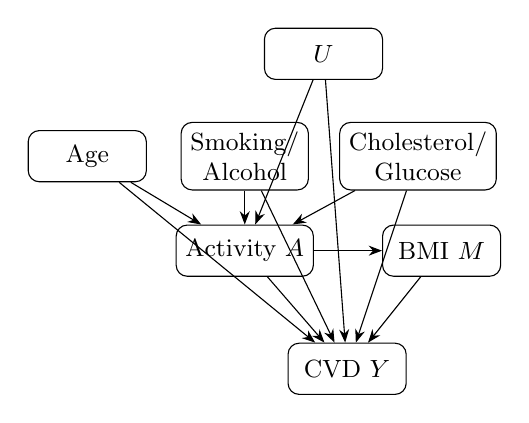
\begin{tikzpicture}[
  >=Stealth, every node/.style={font=\small},
  var/.style={draw, rounded corners, minimum width=1.5cm, minimum height=0.65cm, align=center}
]
  \node[var] (U) at (0,2.3) {$U$};
  \node[var] (age) at (-3,1) {Age};
  \node[var] (beh) at (-1,1) {Smoking/\\Alcohol};
  \node[var] (meta) at (1.2,1) {Cholesterol/\\Glucose};
  \node[var] (A) at (-1,-0.2) {Activity $A$};
  \node[var] (M) at (1.5,-0.2) {BMI $M$};
  \node[var] (Y) at (0.3,-1.7) {CVD $Y$};
  \draw[->] (U) -- (A); \draw[->] (U) -- (Y);
  \draw[->] (age) -- (A); \draw[->] (age) -- (Y);
  \draw[->] (beh) -- (A); \draw[->] (beh) -- (Y);
  \draw[->] (meta) -- (A); \draw[->] (meta) -- (Y);
  \draw[->] (A) -- (Y); \draw[->] (A) -- (M); \draw[->] (M) -- (Y);
\end{tikzpicture}
\caption{Causal DAG. $L$ includes age, sex, smoking, alcohol, cholesterol, glucose, and BMI (total-effect model); mechanism analysis separates BMI as $M$ from $L$.}
\label{fig:dag}
\end{figure}

\section{Identification Assumptions and Estimation Principles}

Identifying ACE from observational data requires assumptions linking potential outcomes to observed variables; only when these hold (or approximately hold) do IPW, g-formula, and propensity score methods receive causal interpretation \cite{hernan2024whatif}. This section explains the meaning of identification assumptions and their correspondence in our data, then describes how each estimator is constructed and why they should yield similar answers.

\subsection{Identification Assumptions}

Consistency requires that for each individual, if observed treatment is $A=a$, then observed outcome $Y$ equals potential outcome $Y(a)$, i.e., $Y=Y(A)=\sum_a Y(a)I(A=a)$ \cite{hernan2024whatif}. Here, $A$ is binary self-reported activity and $Y$ is CVD diagnosis; consistency implies the definition of ``activity'' is unambiguous between potential outcomes and observed variables, with no distinct ``versions'' of treatment for the same $A$ value. Because activity is only a coarse self-reported category, it may encompass different intensities and types; the assumption should be understood as a causal effect of the observed active/inactive label, not of a specific exercise prescription (e.g., 150 minutes MVPA per week) \cite{mi2025creview}.

The stable unit treatment value assumption (SUTVA) comprises no interference and treatment-variation irrelevance \cite{hernan2024whatif}. No interference requires individual $i$'s potential outcomes depend only on $A_i$, not others' treatment; in cross-sectional examination data, inter-individual influence on activity is typically weak, so this assumption is relatively plausible. Treatment-variation irrelevance requires $Y(1)$ and $Y(0)$ to be well defined---if ``active'' means very different activity patterns across individuals, interpretability of potential outcomes declines. Consistency and SUTVA together ensure I estimate a well-defined $\E[Y(1)-Y(0)]$, not an associational contrast confounded by measurement error and definitional drift.

Conditional exchangeability (also ignorability or ``no unmeasured confounding'') is the core of observational causal inference: after controlling $L$, potential outcomes are independent of treatment,
\[
Y(1),Y(0)\indep A\mid L.
\]
This means that within subpopulations with the same $L$, active versus inactive individuals are approximately comparable, as if conditionally randomized within that stratum \cite{hernan2024whatif,rosenbaum1983central}. In Figure~\ref{fig:dag}, $L$ blocks backdoor paths such as $A\leftarrow L\to Y$; if additionally $U\to A$ and $U\to Y$ with $U$ unmeasured, exchangeability fails in the true data-generating mechanism, and identification proceeds only under the untestable premise that $L$ is sufficient \cite{hernan2024whatif}. I limit measured $L$ to age, sex, smoking, alcohol, cholesterol, glucose, and BMI, acknowledging that family history, diet, socioeconomic status, and other $U$ may still threaten identification---Section~7 E-value analysis quantifies how strong such residual confounding would need to be to explain away the estimate \cite{vanderweele2017evalue}.

Positivity (overlap) requires that on the support of $L$,
\[
0<\P(A=1\mid L=l)<1,
\]
i.e., for each covariate profile, both active and inactive individuals exist \cite{hernan2024whatif,chen2024iptw}. If for some $l$, $\P(A=1\mid L=l)\approx 1$, then $\E[Y(0)]$ lacks empirical support in that stratum, IPW weights $1/(1-e(L))$ explode, and matching finds no controls. Positivity differs from exchangeability: the former is directly diagnosable via propensity score distributions and balance plots (Sections~4--5), the latter cannot be proven from data. With 80.3\% active in our sample, positivity faces the reality of high treated proportion and a relatively narrow common support region, but this does not necessarily violate the assumption---the key is whether $\hat e(L)$ overlaps between treated and control groups.

\subsection{Estimation Principles}

Under consistency, SUTVA, $Y(a)\indep A\mid L$, and positivity, average potential outcomes are identified as
\[
\E[Y(a)]=\E\left[\E[Y\mid A=a,L]\right]=\E\left[\frac{I(A=a)\,Y}{\P(A=a\mid L)}\right],
\]
the right-hand side corresponding to outcome regression (g-formula) and inverse probability weighting (IPW) \cite{hernan2024whatif}. Both estimate the same $\E[Y(a)]$ but use data differently: the former models $Y$ then marginalizes over $L$; the latter models $A$ then reweights the sample.

The intuition of IPW is to construct a pseudo-population where $A$ and $L$ are independent \cite{chen2024iptw}. Let $e(L)=\P(A=1\mid L)$; then
\[
\E[Y(a)]=\E\left[\frac{I(A=a)\,Y}{\P(A=a\mid L)}\right]
\]
In finite samples, logistic regression estimates $\hat e(L)=\widehat{\P}(A=1\mid L)$. For $A_i=1$, stabilized weights are often $w_i=\hat P(A=1)/\hat e(L_i)$; for $A_i=0$, $w_i=(1-\hat P(A=1))/(1-\hat e(L_i))$ to reduce weight variance \cite{chen2024iptw}. ACE is the weighted risk difference between active and control groups. IPW requires only the propensity model $\hat e(L)$ to be correct (or close), not the outcome model; but when $e(L)$ is near 0 or 1, weights become extreme and variance increases---hence the importance of positivity diagnostics \cite{chen2024iptw,hernan2024whatif}.

Parametric g-formula standardizes directly over $L$ \cite{hernan2024whatif}:
\[
\E[Y(a)]=\sum_l \E[Y\mid A=a,L=l]\,\P(L=l),
\]
In practice, logistic/linear models fit $\widehat{\E}[Y\mid A,L]$, then average over the sample distribution of $L$. G-formula does not rely on propensity scores, but misspecification of $\E[Y\mid A,L]$ (e.g., ignoring nonlinearity or interactions) still induces bias. When IPW and g-formula both have correct models under positivity, they converge to the same ACE; substantial disagreement often indicates severe misspecification of at least one model \cite{shahu2023comparison}.

Doubly robust augmented IPW (AIPW) combines outcome regression and IPW \cite{robins1994estimation,hernan2024whatif}. Let $\mu(a,L)=\E[Y\mid A=a,L]$; the individual-level estimator is
\[
\hat\psi(a)=\hat\mu(a,L)+\frac{I(A=a)\bigl(Y-\hat\mu(a,L)\bigr)}{\hat e(L)},\qquad
\widehat{\mathrm{ACE}}=\overline{\hat\psi(1)}-\overline{\hat\psi(0)}.
\]
Doubly robustness means: if $\hat e(L)$ is correct, the IPW residual term corrects errors in $\hat\mu$; if $\hat\mu(a,L)$ is correct, then even if $\hat e$ is wrong, $\E[\hat\psi(a)]$ still equals $\E[Y(a)]$ \cite{robins1994estimation,shahu2023comparison}. When a single linear/logistic model may misspecify $e(L)$ or $\mu(a,L)$ in high-dimensional $L$, AIPW provides additional assurance---motivating our reporting of IPW, g-formula, and AIPW together.

The propensity score $\pi(L)=\P(A=1\mid L)$ compresses multidimensional $L$ to one dimension \cite{rosenbaum1983central}. Rosenbaum and Rubin show: if $Y(a)\indep A\mid L$, then $Y(a)\indep A\mid \pi(L)$. Matching compares $Y$ between treated and control with similar $\hat\pi(L)$; stratification divides the sample into propensity quantile groups, estimates effects within groups, then combines with weights \cite{rosenbaum1983central,chen2024iptw}. Like IPW, both aim to block backdoor paths but implement differently: matching/stratification emphasize local comparability; IPW emphasizes global reweighting. I use 1:1 nearest-neighbor matching (caliper$=0.2\times$SD($\hat\pi$)) and quintile stratification to test whether ACE depends on a specific weighting scheme \cite{rosenbaum1983central}. Linear probability models (LPM) regress $Y$ on $A$ controlling $L$; when $\mu(1,L)-\mu(0,L)$ is linear and exchangeability holds, LPM also identifies ACE, often close to g-formula, but lacks AIPW's double robustness \cite{hernan2024whatif}.

In summary, Section~3 reports crude risk difference, IPW, g-formula, AIPW, LPM, PS matching, and PS stratification---all targeting $\mathrm{ACE}=\E[Y(1)-Y(0)]$ under identification assumptions. Convergence across methods supports a narrative of consistent bias direction and adequate adjustment; divergence suggests model or positivity problems \cite{shahu2023comparison,hernan2024whatif}.

\section{Total Effect Estimation and Interpretation}

Section~2 shows that under identification assumptions, ACE can be estimated via IPW, g-formula, AIPW, and PS methods; this section is the core empirical component---first reporting crude and adjusted ACE, then testing convergence across seven methods. If they converge, effect direction and magnitude are insensitive to estimation strategy; Section~4 further asks whether this convergence rests on testable conditions such as positivity.

\subsection{Crude Comparison and the Need for Adjustment}

Before adjustment, the inactive group ($A=0$, $n=13{,}471$) has CVD rate 53.3\%; the active group ($n=54{,}921$) has 48.5\%. The crude risk difference is
\[
\mathrm{ACE}_{\text{crude}}=\bar Y_{A=1}-\bar Y_{A=0}=-0.0476\quad[{-0.0570},\ {-0.0382}],
\]
with 95\% CI excluding zero---the associational difference is statistically significant. Lower CVD rate among active individuals aligns directionally with protective associations summarized by Garcia et al.\ \cite{garcia2023meta} and Mi et al.\ \cite{mi2025creview}; but crude comparison mixes two non-exchangeable sources: backdoor bias from $L$, and selective entry into activity.

Pre-weighting covariate differences (Table~\ref{tab:balance}, left column) show the active group has SMD of $+0.065$ for smoking and $+0.064$ for alcohol, slightly lower BMI (SMD $=-0.035$), slightly lower age (SMD $=-0.026$), and slightly higher cholesterol (SMD $=+0.022$). Smoking and alcohol increase CVD risk yet are more prevalent among active individuals---without controlling $L$, active-group CVD risk is artificially elevated, so crude effects may underestimate true protection (absolute value too large). Slightly lower BMI works in the opposite direction, partially offsetting this bias. Net effect: crude $|\mathrm{ACE}|$ is slightly larger than adjusted, consistent with qualitative predictions from the backdoor structure, showing crude estimates cannot serve as causal conclusions and adjustment is necessary.

\begin{table}[H]
\centering
\caption{Absolute SMD for major covariates before and after IPW weighting}
\label{tab:balance}
\begin{tabular}{lcc}
\toprule
Variable & Before $|\mathrm{SMD}|$ & After $|\mathrm{SMD}|$ \\
\midrule
Smoking     & 0.065 & $<0.001$ \\
Alcohol     & 0.065 & $<0.001$ \\
BMI         & 0.035 & 0.003 \\
Age         & 0.026 & $<0.001$ \\
Cholesterol & 0.022 & $<0.001$ \\
\bottomrule
\end{tabular}
\end{table}

\subsection{ACE Estimates from Seven Methods}

After controlling $L$, Table~\ref{tab:est} and Figure~\ref{fig:forest} summarize seven ACE estimates. By estimation principle: weighting/regression methods (IPW, AIPW, g-formula, LPM) yield $-0.0439$ to $-0.0441$; PS matching $-0.0435$ (SE$=0.0030$, narrowest); PS stratification $-0.0466$ (SE$=0.0077$, widest). Point estimates fall within a 3 percentage-point band $[-0.047,\,-0.044]$, and all 95\% CIs exclude zero---the primary empirical finding: different uses of $\hat e(L)$ and $\E[Y\mid A,L]$ do not produce divergent conclusions, and the protective effect is statistically robust.

\begin{table}[H]
\centering
\caption{ACE of physical activity on CVD ($N=68{,}392$)}
\label{tab:est}
\begin{tabular}{lcc}
\toprule
Method & ACE & 95\% CI \\
\midrule
Crude risk difference  & $-0.0476$ & [$-0.0570$, $-0.0382$] \\
IPW                    & $-0.0440$ & [$-0.0527$, $-0.0354$] \\
Doubly robust AIPW     & $-0.0439$ & [$-0.0520$, $-0.0358$] \\
G-formula              & $-0.0439$ & [$-0.0530$, $-0.0349$] \\
LPM regression         & $-0.0441$ & [$-0.0530$, $-0.0352$] \\
PS matching            & $-0.0435$ & [$-0.0494$, $-0.0376$] \\
PS stratification      & $-0.0466$ & [$-0.0616$, $-0.0315$] \\
\bottomrule
\end{tabular}
\end{table}

\begin{figure}[H]
\centering
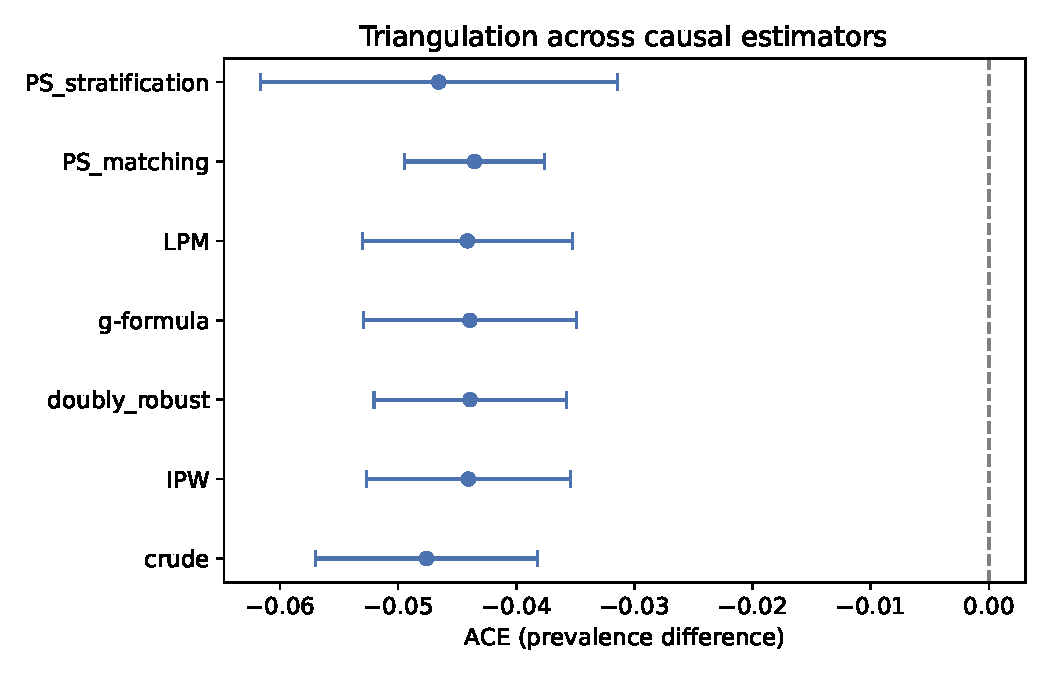
\includegraphics[width=0.88\textwidth]{../figures/forest_plot.pdf}
\caption{Forest plot of seven ACE estimates (horizontal axis: risk difference; vertical lines: 95\% confidence intervals)}
\label{fig:forest}
\end{figure}

Using the IPW point estimate with inactive-group risk $p_0=0.533$ as reference, active-group risk is approximately $p_0+\mathrm{ACE}\approx 0.489$, giving approximate RR $\approx 0.92$---protective direction consistent with literature, but because the outcome is CVD prevalence rather than mortality and activity is only binary self-report, magnitudes should not be numerically compared directly to Garcia et al.'s \cite{garcia2023meta} CVD death RR (0.71). For this dataset, moving 80.3\% of active individuals from the inactive counterfactual state to active would reduce population-average CVD probability by about 4.4 percentage points, with clear public health interpretability.

\subsection{Why Multiple Methods Converge}

Why do IPW (relying on $\hat e$), g-formula (relying on $\hat\mu$), AIPW (combining both), and PS matching/stratification (relying on local comparability via $\hat\pi$) yield nearly identical ACE? From an identification perspective, all target $\E[Y(1)]-\E[Y(0)]$. Here, IPW and g-formula differ by only 0.0001 ($-0.0440$ vs $-0.0439$), and AIPW coincides exactly---meaning propensity and outcome models do not conflict enough at the ACE level to split conclusions; severe misspecification of one typically separates IPW and g-formula \cite{shahu2023comparison}. AIPW not triggering single-model compensation means both working models mutually support---the core value of triangulation: not repeating one regression, but cross-validating the same estimand via different identification paths \cite{shahu2023comparison,hernan2024whatif}.

Method by method: IPW and g-formula correspond to the two formulas in Section~2.2---the former reweights so $A\indep L$, the latter marginalizes $\E[Y\mid A,L]$; equivalence under correct models is empirically reflected here. AIPW is consistent if either $\hat e$ or $\hat\mu$ is correct in the Robins sense \cite{robins1994estimation}; coincidence with IPW indicates at least not the worst case of both models failing. LPM coefficient $-0.0441$ nearly equals g-formula, as expected under linear $\E[Y\mid A,L]$ \cite{hernan2024whatif}.

PS matching ($-0.0435$) is slightly smaller in magnitude than IPW ($-0.0440$) with narrower SE (0.0030 vs 0.0044), consistent with ``local randomization'' among similar $\hat\pi$ and exclusion of non-comparable individuals outside the caliper---the matched sample is more homogeneous, estimates are more precise, but may slightly deviate from the full-sample ACE. PS stratification ($-0.0466$) has the point estimate closest to crude and the widest interval, because $A=0$ individuals are sparse within quintile strata and within-stratum variance is large---directly related to narrow positivity under high activity prevalence (Section~4). Nevertheless, stratification still falls within other methods' CIs, showing the effect is not an artifact of one weighting scheme.

The difference between crude and adjusted ACE ($-0.0476$ vs $-0.0440$) is also understandable from the backdoor structure: after controlling $L$, smoking/alcohol's upward pull on active-group CVD risk is removed, and ACE absolute value slightly decreases, consistent with Section~3.1 confounding direction. In sum, multi-method triangulation supports: under control of $L$ and identification assumptions, activity reduces average CVD risk by about 4.4 percentage points. But convergence alone does not prove positivity or exchangeability---Section~4 turns to positivity, the only assumption in Section~2.1 that is testable from data.

\section{Positivity Assessment: Propensity Score Overlap}

Section~3 ACE estimates rely on IPW and PS methods, both requiring positivity: $0<e(L)<1$ on the support of $L$ \cite{hernan2024whatif,chen2024iptw}. If treated and control $\hat e(L)$ barely overlap, then $\E[Y(0)]$ is unidentified in regions lacking controls, and Section~3 numerical agreement may rest on extrapolation rather than identification. This section tests common support via propensity score distributions.

\subsection{Common Support and Distributional Overlap}

Let $\hat e(L)=\widehat{\P}(A=1\mid L)$. Figure~\ref{fig:overlap} shows densities of $\hat e$ for $A=0$ and $A=1$. With 80.3\% active, the logistic propensity model assigns high $\hat e$ to most individuals: inactive group ($n=13{,}471$) mean $\hat e$ 0.802, range $[0.742,\,0.874]$; active group ($n=54{,}921$) mean 0.804, range $[0.745,\,0.879]$. Common support is $\hat e\in[0.745,\,0.874]$; 99.99\% of individuals fall in this interval. Positivity is not empirically violated---at each $\hat e$ level, both active and inactive individuals exist, IPW weights do not systematically explode from complete lack of controls, and PS matching finds controls within the caliper.

\begin{figure}[H]
\centering
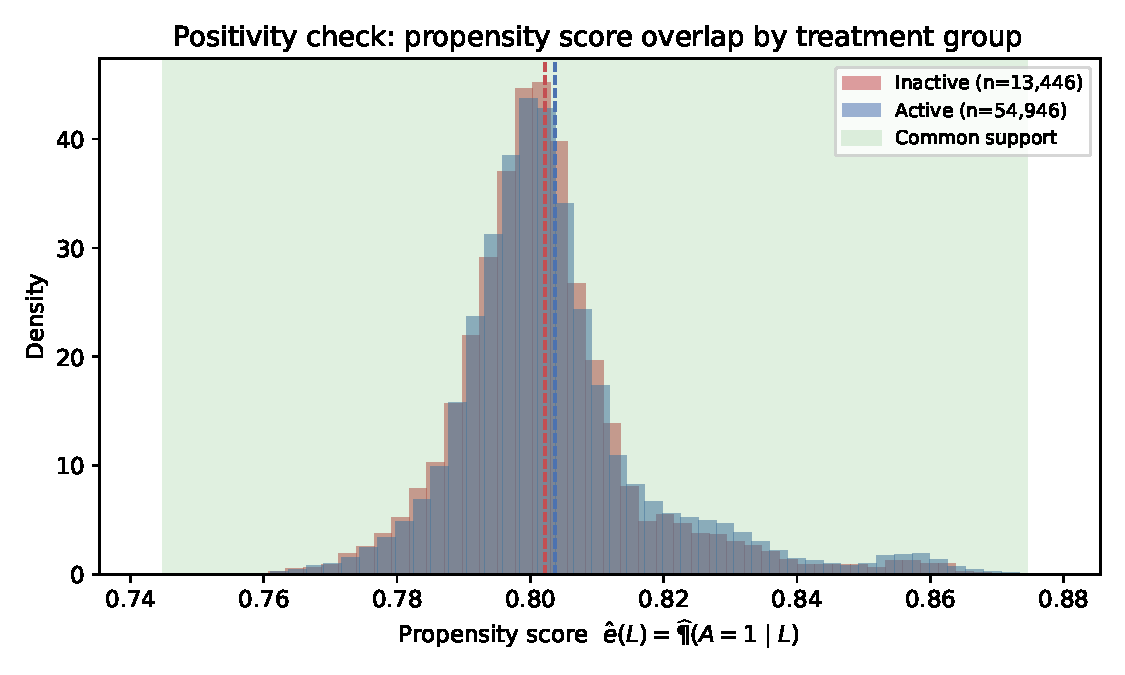
\includegraphics[width=0.92\textwidth]{../figures/ps_overlap.pdf}
\caption{Positivity assessment: propensity score distributions by treatment group and common support region (green). Dashed lines indicate group PS means.}
\label{fig:overlap}
\end{figure}

From weight structure: for inactive individuals, stabilized IPW weight is $w_i=(1-\hat P(A=1))/(1-\hat e(L_i))$ with $\hat P(A=1)=0.803$. At mean $\hat e=0.802$, $w_i\approx 0.197/0.198\approx 1.0$; for active individuals, $w_i=\hat P(A=1)/\hat e(L_i)\approx 0.803/0.802\approx 1.0$. Even at upper common-support bound $\hat e=0.874$, inactive weight is about $0.197/0.126\approx 1.56$, moderate rather than explosive. Section~3 IPW is not dominated by extreme weights---positivity is not only formally satisfied but corresponds to acceptable weight distributions \cite{chen2024iptw}.

Positivity assessment answers whether data contain control information needed to compare $\E[Y(1)]$ and $\E[Y(0)]$, not whether exchangeability holds. Overlap plots at least exclude the most fatal identification failure---complete lack of overlap \cite{chen2024iptw}---providing a necessary (not sufficient) condition for Section~3 IPW/PS estimates.

\subsection{Identification Implications Under High Activity Prevalence}

Structural features of this data must also be noted: group mean $\hat e$ values are nearly identical (0.802 vs 0.804), common support width only about 0.13---almost everyone is predicted ``high activity propensity.'' ACE identification therefore relies mainly on conditional probability variation within $L$ rather than broad dispersion of $\hat e$ near 0. If $L$'s explanatory power for $A$ increases further and $\hat e$ concentrates toward 1, positivity will tighten marginally \cite{chen2024iptw}.

This pattern is consistent with high activity prevalence (80.3\%): marginally only 19.7\% are inactive, but conditionally individuals with $e(L)<1$ may still exist---Figure~\ref{fig:overlap} tests this directly. It explains Section~3's widest PS stratification CI (SE$=0.0077$): in quintile strata, several layers have very few $A=0$ samples and large within-stratum variance; global IPW uses all 13{,}471 inactive individuals as controls, with SE (0.0044) much smaller than PS stratification. If positivity truly failed (e.g., $\hat e\to 1$ with no $A=0$ individuals), I would simultaneously see overlap disappearance, weight explosion, and PS matching failure to pair---patterns not observed here.

The relationship between positivity and Section~3 conclusions: multi-method convergence in Section~3 is obtained under the premise that IPW/PS identification is feasible within common support; this section excludes the most severe case where estimates rely purely on extrapolation from lack of controls. The next section further tests whether IPW truly balances $L$ within common support (Table~\ref{tab:balance} already previews post-weighting $|\mathrm{SMD}|<0.003$), verifying backdoor blocking in data.

\section{Covariate Balance and IPW Validity}

Section~4 shows positivity holds in data, giving IPW/PS estimates the necessary conditions for identification. But positivity only guarantees controls exist, not that IPW weights eliminate distributional differences in $L$ between treated and control---if $L$ remains imbalanced after weighting, backdoor blocking implied by $Y(a)\indep A\mid L$ fails at the data level and Section~3 ACE may still suffer residual confounding \cite{rosenbaum1983central,chen2024iptw}. This section quantifies covariate balance before and after IPW via love plots and SMD, testing whether Section~2.2 IPW ``pseudo-randomization'' is achieved on measured $L$.

\subsection{Balance Principle of IPW Weighting}

Rosenbaum and Rubin's \cite{rosenbaum1983central} core result: if $Y(a)\indep A\mid L$, then $Y(a)\indep A\mid \pi(L)$ where $\pi(L)=\P(A=1\mid L)$. Further, within strata of similar propensity scores, $L$ distributions should approximate balance between treated and control---the testable implication of IPW validity \cite{chen2024iptw}. With stabilized weights $w_i$ as in Section~2.2, post-weighting standardized mean difference (SMD) for covariate $j$ is
\[
\mathrm{SMD}_j=\frac{\bar L_{j,A=1}^{w}-\bar L_{j,A=0}^{w}}{s_j},
\]
where $\bar L^w$ is the weighted mean and $s_j$ the pooled standard deviation. Empirically $|\mathrm{SMD}|<0.1$ is acceptable balance \cite{chen2024iptw}; post-weighting $|\mathrm{SMD}|>0.1$ suggests omitted covariates in the propensity model, positivity only in a narrow region, or insufficient IPW weighting \cite{chen2024iptw,hernan2024whatif}.

Balance diagnostics test whether backdoor paths on measured $L$ are blocked, not whether exchangeability holds. With unobserved $U$, even perfect balance on $L$ may leave $Y(a)\indep A\mid L$ violated---Section~7 E-value quantifies how strong $U$ would need to be to explain away Section~3 estimates \cite{vanderweele2017evalue}.

\Needspace{14cm}
\subsection{Covariate Differences Before and After Weighting}

Table~\ref{tab:balance_full} and Figure~\ref{fig:love} report SMD for seven adjustment covariates. Before weighting, active and inactive groups differ systematically: smoking ($|\mathrm{SMD}|=0.065$) and alcohol (0.065) show the largest differences, with higher prevalence among active individuals---consistent with Section~3.1 confounding direction; BMI (0.035), age (0.026), cholesterol (0.022), glucose (0.020) also differ visibly; sex (0.014) is smallest but nonzero. These differences explain why crude and adjusted ACE differ: without weighting, backdoor paths $A\leftarrow L\to Y$ are not blocked \cite{hernan2024whatif}.

After IPW weighting, all seven covariates have $|\mathrm{SMD}|<0.003$ (gender 0.001, smoke/alco $<0.001$, BMI 0.003, gluc 0.002, age/cholesterol $<0.001$). Maximum imbalance compresses from 0.065 to under 0.003, a reduction exceeding 95\%. In the pseudo-population, $A$ and $L$ are approximately independent, showing the logistic propensity model $\hat e(L)$ successfully achieves post-weighting covariate balance---direct evidence that IPW operates effectively as a backdoor adjustment tool \cite{chen2024iptw}.

\begingroup
\setlength{\intextsep}{6pt plus 2pt minus 2pt}
\begin{samepage}
\begin{table}[H]
\centering
\caption{SMD for all adjustment covariates before and after IPW weighting}
\label{tab:balance_full}
\begin{tabular}{lrr}
\toprule
Variable & Pre-weight SMD & Post-weight SMD \\
\midrule
Smoking (smoke)     & $+0.065$ & $-0.000$ \\
Alcohol (alco)      & $+0.065$ & $-0.000$ \\
BMI                 & $-0.035$ & $-0.003$ \\
Age                 & $-0.026$ & $-0.000$ \\
Cholesterol         & $+0.022$ & $+0.000$ \\
Glucose (gluc)      & $-0.020$ & $-0.002$ \\
Sex (gender)        & $+0.014$ & $+0.001$ \\
\bottomrule
\end{tabular}
\end{table}
\vspace{-0.3em}
\begin{figure}[H]
\centering
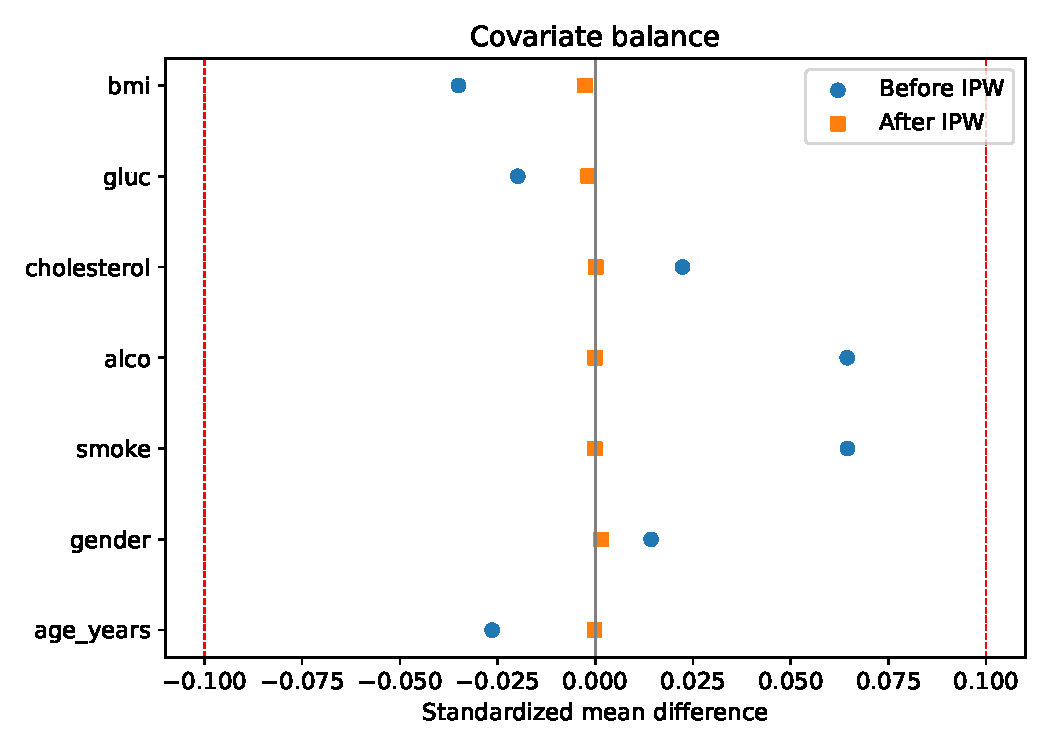
\includegraphics[width=0.72\textwidth]{../figures/love_plot.pdf}
\caption{Covariate SMD before and after IPW weighting. Red dashed lines indicate $\pm 0.1$ thresholds.}
\label{fig:love}
\end{figure}
\end{samepage}
\endgroup

\subsection{Implications of Balance Diagnostics for Section~3 ACE}

Linking Sections~4--5 diagnostics with Section~3 conclusions forms a complete testable evidence chain: Section~4 positivity shows common support holds (99.99\% in $\hat e\in[0.745,0.874]$), IPW weights do not explode (inactive weight $\approx 1.56$ at upper bound); this section's love plot shows good post-weighting balance on $L$. Together they support that Section~3 IPW ACE $=-0.0440$ is not a spurious estimate under lack of controls or severe post-weighting imbalance \cite{hernan2024whatif,chen2024iptw}.

Good balance does not prove $U$ is absent. Smoking/alcohol---``negative health behaviors'' slightly more common among active individuals---are balanced by IPW; but unmeasured $U$ (family history, diet) correlated with both activity and CVD may still violate exchangeability. Positivity and balance exclude the most severe identification failures at the testable level; Section~6 examines mechanisms given stable total effects, and Section~7 further bounds conclusion strength via adjustment specifications and E-value \cite{vanderweele2017evalue}.

\section{Mechanism Analysis: BMI Mediation Path}

Sections~3--5 establish that after controlling $L$, total effect ACE $\approx -0.044$, with IPW identification conditions verified in data. The next question: how much of this protective effect passes through BMI? Chen and Wang et al.\ report PA mediation through obesity-related indices among Chinese adults and in recreational activity--hypertension studies \cite{chen2023pa,wang2023obesity}; Hall et al.\ \cite{bjsports2023crf} note more complex mechanisms when considering CRF. This section, under VanderWeele's regression-based mediation framework \cite{vanderweele2015explanation}, separates BMI from $L$ as mediator $M$, decomposing NDE and NIE, with comparison to concurrent blood pressure mediation and sensitivity analysis.

\subsection{Mediation Estimands and Identification Framework}

In Figure~\ref{fig:dag}, the total-effect model includes BMI in $L$ to block backdoor path $A\leftarrow M\to Y$; mechanism analysis requires a different estimand: controlling $L\setminus\{M\}=\{$age, sex, smoking, alcohol, cholesterol, glucose$\}$, define
\[
\mathrm{NDE}=\E[Y(1,M(0))-Y(0,M(0))],\qquad
\mathrm{NIE}=\E[Y(0,M(1))-Y(0,M(0))],
\]
with total effect $\mathrm{TE}=\mathrm{NDE}+\mathrm{NIE}$ \cite{vanderweele2015explanation}. NDE is the effect of activity on CVD when the $A\to M$ path is blocked; NIE is the effect transmitted only through BMI change. Under linear LPM approximation, decomposition uses $a$- and $b$-paths:
\[
\mathrm{NIE}=a\times b,\quad
a=\E[M(1)-M(0)\mid L\setminus M],\quad
b=\E[Y(1,m)-Y(0,m)\mid L\setminus M,\,M=m].
\]
Identification requires additional assumptions: no unmeasured confounders between $M$ and $Y$, $L\setminus M$ sufficiently controls confounding for $A$--$M$ and $A$--$Y$, and cross-world independence \cite{vanderweele2015explanation}. A single cross-sectional BMI measurement cannot capture dynamic weight change---limitations to remember when interpreting NIE proportion.

\subsection{BMI Path Decomposition Results}

Table~\ref{tab:med} summarizes decomposition (500 bootstrap CIs). $a$-path coefficient $-0.183$: active individuals have mean BMI 0.18 units lower (approximately 0.18 kg/m$^2$), confirming activity associates with lower BMI. $b$-path $+0.014$: controlling $L\setminus M$, each 1-unit BMI increase raises CVD risk difference by 1.4 percentage points. Product $\mathrm{NIE}=-0.183\times 0.014\approx -0.0026$ [$-0.0040$, $-0.0013$]: activity indirectly lowers CVD risk through BMI by about 0.26 percentage points. $\mathrm{NDE}=-0.0441$ [$-0.0530$, $-0.0362$], about 94\% of total effect $\mathrm{TE}=-0.0468$ [$-0.0562$, $-0.0383$]; indirect path about 5.6\%.

\begin{table}[H]
\centering
\caption{BMI mediation path decomposition (controlling $L\setminus M$: age, sex, smoking, alcohol, cholesterol, glucose)}
\label{tab:med}
\begin{tabular}{lcc}
\toprule
Effect / path & Estimate & 95\% CI \\
\midrule
$a$-path ($A\to M$)           & $-0.183$ & --- \\
$b$-path ($M\to Y\mid A$)    & $+0.014$ & --- \\
NIE (indirect effect)         & $-0.0026$ & [$-0.0040$, $-0.0013$] \\
NDE (direct effect)           & $-0.0441$ & [$-0.0530$, $-0.0362$] \\
Total effect TE               & $-0.0468$ & [$-0.0562$, $-0.0383$] \\
Indirect effect proportion    & 5.6\% & --- \\
\bottomrule
\end{tabular}
\end{table}

\begin{figure}[H]
\centering
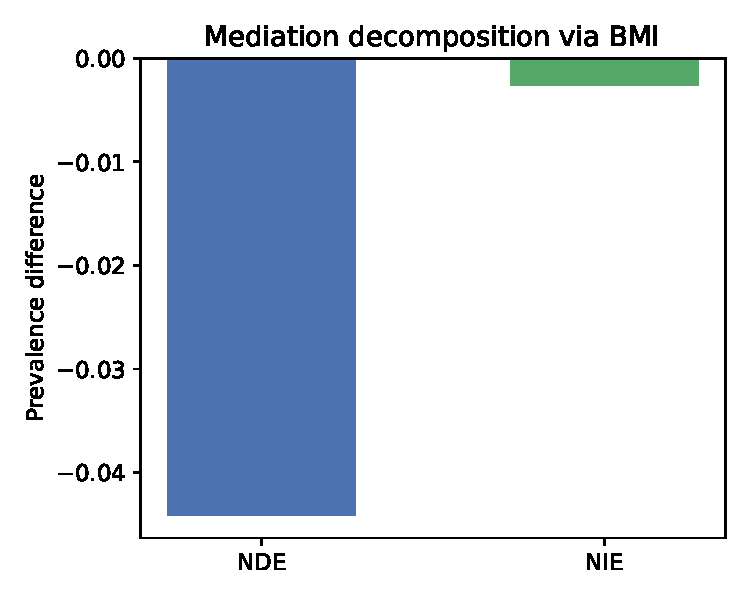
\includegraphics[width=0.48\textwidth]{../figures/mediation_decomp.pdf}
\hfill
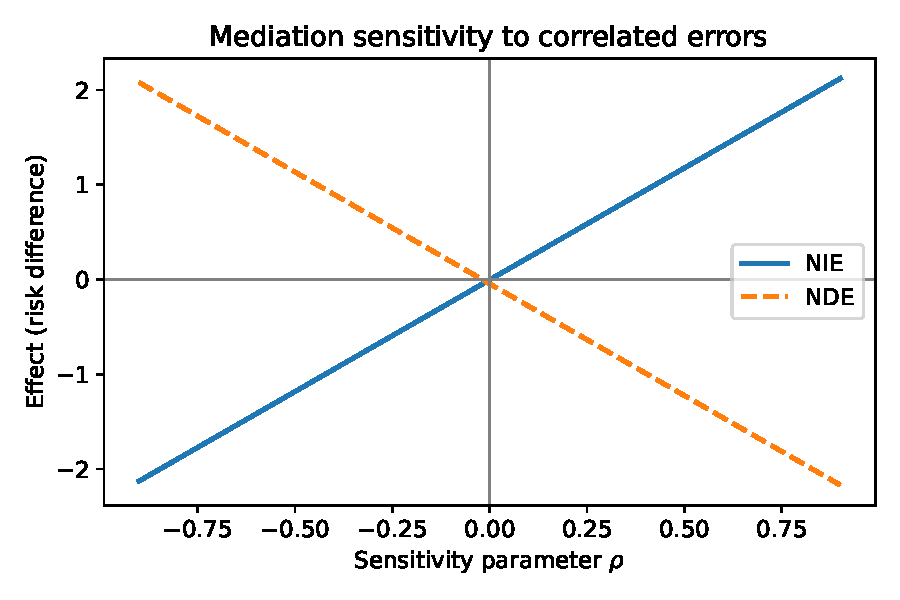
\includegraphics[width=0.48\textwidth]{../figures/mediation_sensitivity.pdf}
\caption{Left: NDE and NIE decomposition; right: mediation sensitivity---NIE change as $\rho$ (correlation of mediator/outcome model residuals) varies}
\label{fig:med}
\end{figure}

Figure~\ref{fig:med} (left) visually shows NDE dominance. Compared with Section~3: IPW total effect excluding BMI as confounder is $-0.0468$ (Section~7), matching mediation TE $=-0.0468$---because BMI is no longer controlled as confounder in the mechanism model, total effect is slightly larger than main-analysis ACE ($-0.0440$), consistent with DAG expectations when BMI is both confounder and mediator \cite{vanderweele2015explanation}. NDE $=-0.0441$ nearly equals main-analysis LPM/IPW, meaning Section~3 total effect is essentially close to the direct effect not passing through BMI; the BMI channel contributes only about 5.6\% additional protection.

\subsection{Comparison with Literature and Blood Pressure Mediation}

Does NDE at 94\% contradict literature? Not necessarily. Chen et al.\ \cite{chen2023pa} report PA mediation through body fat, blood pressure, lipids, and other pathways among Chinese adults---I test only the BMI single path, with cross-sectional binary activity; the $a$-path is significant but limited in magnitude. Biologically, activity may also affect CVD through endothelial function, systemic inflammation, cardiorespiratory fitness, etc., not necessarily via BMI \cite{bjsports2023crf,srep2025stiffness}. Wang et al.\ \cite{wang2023obesity} find obesity indices mediate PA--hypertension associations, but our outcome is CVD not hypertension, and BMI is only a coarse obesity proxy.

As design contrast, replacing mediator with concurrent systolic pressure $ap\_hi$ yields $\mathrm{NIE}=+0.0006$, $\mathrm{NDE}=-0.0447$, total effect $=-0.0441$---indirect path nearly zero. This is not because blood pressure is unimportant, but because cross-sectional blood pressure reflects both long-term activity effects and prevalent cardiovascular pathology; a single examination cannot identify the dynamic chain activity$\to$blood pressure change$\to$CVD \cite{srep2025stiffness,hernan2024whatif}. This does not contradict significant blood pressure mediation in longitudinal cohorts, but again exposes cross-sectional design limits.

\subsection{Mediation Sensitivity Analysis}

Figure~\ref{fig:med} (right) reports VanderWeele-style sensitivity \cite{vanderweele2015explanation}: if unmeasured factors correlate mediator and outcome model residuals (parameter $\rho$), NIE rises with $\rho$. Here, mediator/outcome residual SDs are 5.02 and 0.47; at $\rho\approx 0.001$, NIE is fully offset ($\rho_{\text{tip}}\approx 0.0011$). Because NIE itself is only 5.6\%, small $\rho$ can flip the indirect effect---mainly threatening mechanism interpretation (``does activity work through BMI?'') rather than total effect: scanning $\rho$, NDE remains stable around $-0.044$, consistent with Section~3 IPW ACE. Thus, the conclusion that activity lowers CVD does not depend on BMI mediation; even if NIE is fully explained by unmeasured factors, NDE still supports a protective total effect.

\section{Heterogeneity, Adjustment Specifications, and Unmeasured Confounding}

Section~3 gives overall ACE; Sections~5--6 show identification diagnostics pass and BMI mediation is a small share. This section stress-tests conclusions from three angles: consistency across subgroups (heterogeneity), dependence on adjustment specifications (sensitivity), and strength of unmeasured confounding needed to explain away estimates (E-value). Together they bound extrapolation of Section~3 causal conclusions \cite{vanderweele2017evalue,hernan2024whatif}.

\subsection{Age-Stratified Heterogeneity}

Repeating IPW by age quartiles (Q1 youngest $\to$ Q4 oldest), Figure~\ref{fig:age} (left) reports stratum ACE. Q1: $-0.041$ [$-0.059$, $-0.023$]; Q2: $-0.039$ [$-0.057$, $-0.022$]; Q3: $-0.047$ [$-0.066$, $-0.029$]; Q4: $-0.050$ [$-0.068$, $-0.031$]. All four 95\% CIs exclude zero and overlap substantially---protective effects exist across age groups without statistically significant effect modification.

Age-stratified IPW re-estimates $\hat e(L)$ and ACE within each stratum, testing whether protection is driven by one age group. Q4 point estimate is slightly larger ($-0.050$ vs Q2 $-0.039$), possibly because older groups have higher baseline CVD risk and greater absolute risk reduction space from activity \cite{mi2025creview}; but within-stratum sample sizes are smaller than full sample, SE about 0.009 (full-sample IPW SE 0.004), CIs are wider, insufficient to assert significant heterogeneity. This supports that full-sample Section~3 ACE is not an artifact of one age stratum but a protective direction across the life course.

\subsection{Effect Modification by Smoking}

Adding activity$\times$smoking interaction in LPM (controlling remaining $L\setminus\{\text{smoke}\}$), Figure~\ref{fig:age} (right) reports stratum effects. Non-smokers: ACE $-0.0417$ [$-0.0510$, $-0.0324$]; smokers: $-0.0734$ [$-0.1079$, $-0.0389$]; interaction coefficient $-0.032$, $p=0.062$, marginally significant.

Smokers have higher baseline CVD risk (smoking is a strong risk factor in $L$), so larger absolute risk reduction from activity in that subgroup is not surprising \cite{medrxiv2023genePA}. But smoker CI is wide (upper bound $-0.039$ still significantly negative, lower bound $-0.108$ indicates large uncertainty), and $p=0.062$ does not reach conventional 0.05---I treat this as an exploratory finding, not asserting activity is more effective for smokers. Importantly, among non-smokers alone, ACE remains $-0.042$ and significant; Section~3 conclusions do not depend on smoking interaction.

\begin{figure}[H]
\centering
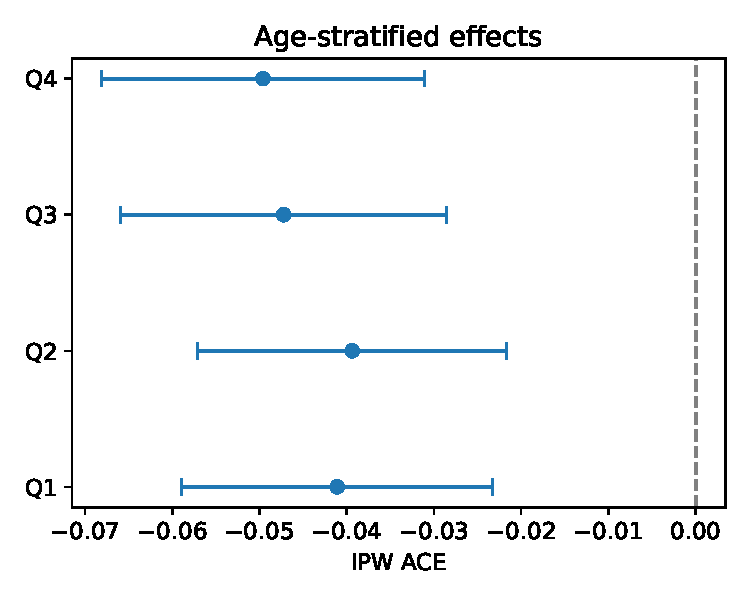
\includegraphics[width=0.46\textwidth]{../figures/age_heterogeneity.pdf}
\hfill
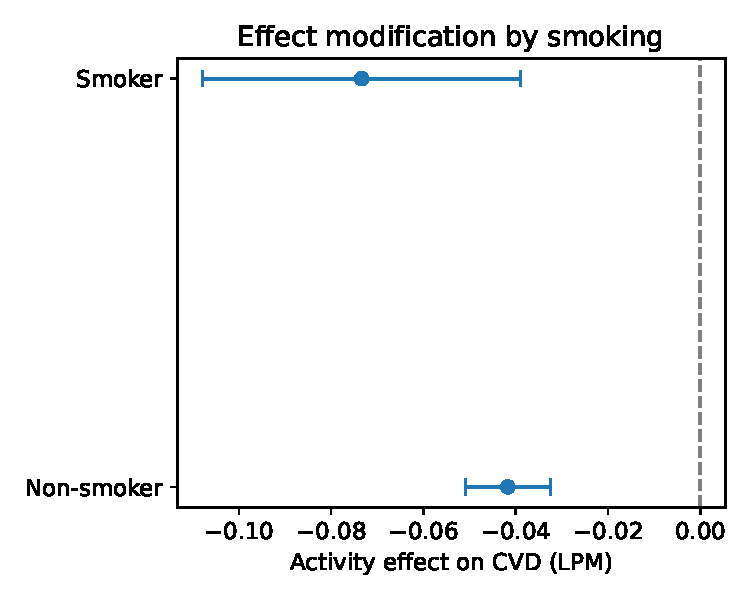
\includegraphics[width=0.46\textwidth]{../figures/effect_modification.pdf}
\caption{Left: IPW ACE by age quartile with 95\% CIs; right: LPM effects stratified by smoking with 95\% CIs}
\label{fig:age}
\end{figure}

\subsection{Adjustment Set Specification Sensitivity}

Adjustment set choice directly changes estimand meaning \cite{vanderweele2015explanation,hernan2024whatif}. Figure~\ref{fig:adj} compares three IPW specifications (Table~\ref{tab:adj}): main analysis (with BMI) ACE $=-0.0440$ [$-0.0534$, $-0.0347$]; excluding BMI $-0.0468$ [$-0.0557$, $-0.0379$]; additionally including systolic/diastolic pressure $-0.0446$ [$-0.0530$, $-0.0361$].

\begin{table}[H]
\centering
\caption{IPW ACE under different adjustment sets}
\label{tab:adj}
\begin{tabular}{lcc}
\toprule
Specification & ACE & 95\% CI \\
\midrule
Main analysis ($L$ includes BMI)              & $-0.0440$ & [$-0.0534$, $-0.0347$] \\
Exclude BMI                                   & $-0.0468$ & [$-0.0557$, $-0.0379$] \\
Add blood pressure ($ap\_hi$, $ap\_lo$)       & $-0.0446$ & [$-0.0530$, $-0.0361$] \\
\bottomrule
\end{tabular}
\end{table}

\begin{figure}[H]
\centering
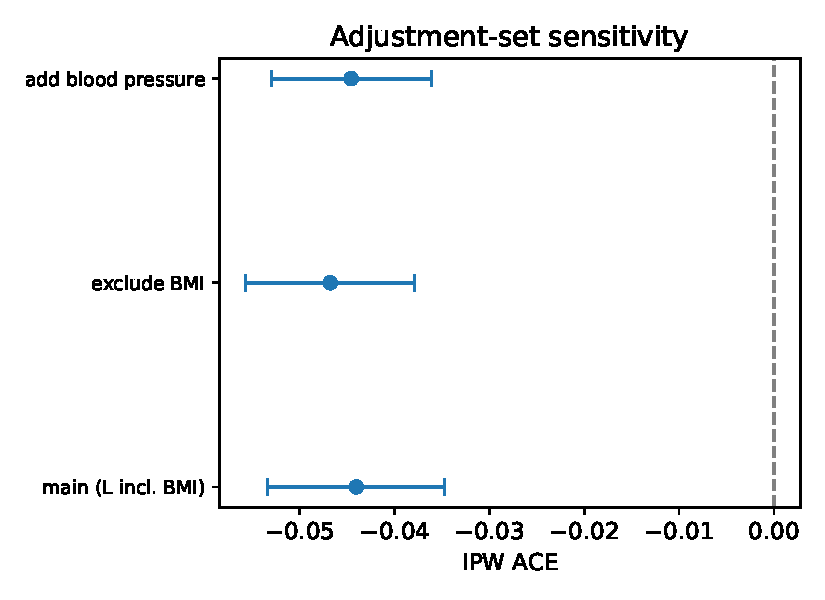
\includegraphics[width=0.65\textwidth]{../figures/adjustment_sensitivity.pdf}
\caption{IPW ACE and 95\% CIs under different adjustment sets}
\label{fig:adj}
\end{figure}

Excluding BMI increases ACE magnitude by about 0.003, consistent with Section~6 mechanism analysis: BMI is both confounder on $A\to Y$ and mediator on $A\to M\to Y$; main analysis controlling BMI estimates total effect including BMI confounding paths; excluding BMI partially opens mediation paths, shifting TE toward $-0.0468$ \cite{vanderweele2015explanation}. Adding blood pressure barely changes ACE ($-0.0446$ vs $-0.0440$), showing concurrent blood pressure does not strongly drive conclusions---neither supporting ``must control blood pressure'' nor extreme ``effect greatly attenuated after controlling blood pressure,'' consistent with Section~1 design choice not to control blood pressure in main analysis \cite{hernan2024whatif}. All three specifications' CIs overlap substantially; Section~3 ACE is robust to reasonable adjustment changes.

\subsection{E-Value and Unmeasured Confounding}

Exchangeability $Y(a)\indep A\mid L$ is untestable; E-value quantifies how strong unmeasured confounding $U$ would need to be to fully explain away the observed effect \cite{vanderweele2017evalue}. Using IPW point estimate $\mathrm{ACE}=-0.0440$ and inactive-group CVD rate $p_0=0.533$, active-group risk is approximately $p_1\approx 0.489$, giving approximate RR $\approx 0.92$. E-value point estimate is about 1.40; for the lower bound of the 95\% CI on ACE, E-value is about 1.46---meaning if unmeasured $U$ exists, its associations with both activity and CVD (on RR scale) would each need to reach about 1.4 to fully offset the observed protective effect \cite{vanderweele2017evalue}.

An E-value of 1.40 is not high: family history, diet, socioeconomic status, and other $U$ may plausibly reach this magnitude of association with both activity and CVD \cite{mi2025creview,hernan2024whatif}. Thus, even with Section~3--5 multi-method convergence and passing positivity and balance, I position causal conclusions as supportive evidence consistent across methods and diagnostics, not RCT-level confirmation. E-value closes the loop with Section~5's point that $U$ may still threaten exchangeability: testable conditions are good, untestable assumptions require caution.

Linking Section~7 with the full paper: Section~3 ACE is stable; Sections~4--5 testable identification conditions hold; Section~6 mechanisms are NDE-dominated; this section shows effects are robust to age, insensitive to reasonable adjustment changes, but E-value indicates residual confounding cannot be ignored---providing complete basis for Section~8 conclusions and limitations.

\section{Conclusions and Limitations}

\subsection{Main Conclusions}

In observational data, this study conducts a complete causal inference pipeline around whether physical activity causally lowers CVD risk: identification assumptions, multi-method estimation, testable diagnostics, mechanism and sensitivity analysis. Methodologically, under DAG and backdoor guidance I specify the average causal effect estimand, sequentially applying IPW, g-formula, doubly robust AIPW, LPM, and PS matching/stratification---principally different strategies---and testing positivity and covariate balance via propensity score overlap and post-weighting balance; I further decompose BMI mediation under VanderWeele's framework, combining adjustment-set variation, subgroup analysis, and E-value to assess conclusion strength \cite{hernan2024whatif,vanderweele2015explanation,vanderweele2017evalue}.

Main findings summarize as three points. First, after controlling age, sex, smoking, alcohol, and major metabolic indicators, multiple methods agree closely in direction and magnitude on total effect, all supporting a protective association between physical activity and CVD risk---showing conclusions do not depend on one weighting or regression specification but have reasonable methodological robustness under stated assumptions \cite{shahu2023comparison}. Second, positivity and post-IPW covariate balance diagnostics show testable identification conditions are met in data; Section~3 effect estimates do not rest on fragile foundations of lack of controls or severe post-weighting imbalance \cite{chen2024iptw,rosenbaum1983central}. Third, mechanism analysis shows protection operates mainly through direct paths not mediated by BMI, with small indirect share via BMI; effects are protective across age strata and insensitive to reasonable adjustment changes, but E-value analysis indicates unmeasured confounding may still weaken causal interpretation \cite{vanderweele2017evalue}.

In practical terms, conclusions align with Garcia et al.\ \cite{garcia2023meta}, Mi et al.\ \cite{mi2025creview}, and extensive observational evidence that insufficient physical activity is a modifiable CVD risk factor: population-level promotion of regular activity and reduced sedentary behavior retains clear public health value. Beyond a protective point estimate, this paper demonstrates on a single observational dataset how to combine causal estimand specification, multi-method triangulation, and testable diagnostics to make the inference from association to causation transparent and reproducible---a reference for future analyses of similar examination or cohort data.

\subsection{Limitations and Outlook}

Several limitations require attention in interpretation and generalization. Data are cross-sectional, all variables measured at one examination time, so reverse causation (individuals with CVD reducing activity) cannot be excluded; activity is binary self-report without intensity, frequency, or objective measurement, not one-to-one with guideline MVPA dose \cite{mi2025creview}. Exchangeability is fundamentally untestable; despite passing positivity and balance, unmeasured family history, diet, socioeconomic status, etc., may constitute residual confounding, and E-value analysis shows confounding strength needed to fully explain away observed effects is not extreme \cite{vanderweele2017evalue,hernan2024whatif}. Mediation analysis relies on linear approximation and cross-sectional BMI measurement; answers about biological pathways through which activity lowers CVD remain preliminary \cite{vanderweele2015explanation}.

In sum, I position causal conclusions as supportive evidence consistent across methods and diagnostics, not randomized-trial confirmation. Future work may validate in longitudinal follow-up, natural experiments, or instrumental variable/MR designs; combining accelerometer activity measurement with richer covariates could improve estimand interpretability and extrapolation strength. All code, data, figures, and numerical output are public on GitHub (Appendix~\ref{app:repo}) for reproduction and extension.

\clearpage
\centerline{\cfttoctitlefont Appendix}\par
\vspace{1.2em}
\appendix

\section{Figure and Table Index}
\label{app:figures}

Main tables in the text include: Table~\ref{tab:est} (seven ACE estimates), Tables~\ref{tab:balance} and~\ref{tab:balance_full} (covariate balance), Table~\ref{tab:med} (BMI mediation decomposition), Table~\ref{tab:adj} (adjustment sensitivity). Main figures are listed below.

\begin{table}[H]
\centering
\caption{Index of main figures in the text}
\label{tab:figindex}
\begin{tabular}{clp{6.5cm}}
\toprule
Fig. & Filename & Content \\
\midrule
\ref{fig:dag}     & (TikZ)                    & Causal directed acyclic graph \\
\ref{fig:forest}  & \texttt{forest\_plot.pdf} & Forest plot of seven ACE estimates \\
\ref{fig:overlap} & \texttt{ps\_overlap.pdf}  & Propensity score overlap (positivity) \\
\ref{fig:love}    & \texttt{love\_plot.pdf}   & SMD before and after IPW weighting \\
\ref{fig:med}     & \texttt{mediation\_*.pdf} & BMI mediation decomposition and $\rho$ sensitivity \\
\ref{fig:age}     & \texttt{age\_heterogeneity.pdf}, etc. & Age stratification and smoking effect modification \\
\ref{fig:adj}     & \texttt{adjustment\_sensitivity.pdf} & Adjustment set sensitivity \\
\bottomrule
\end{tabular}
\end{table}

\section{Notation}
\label{app:notation}

\small
\begin{longtable}{@{}clp{8.2cm}@{}}
\caption{Summary of main notation used in the text}\label{tab:notation} \\
\toprule
Symbol & Name & Meaning \\
\midrule
\endfirsthead
\multicolumn{3}{c}{\small Table~\thetable{} (continued)} \\
\toprule
Symbol & Name & Meaning \\
\midrule
\endhead
\bottomrule
\endfoot
\bottomrule
\endlastfoot
$N$ & Sample size & Analysis sample after cleaning ($N=68{,}392$) \\
$n$ & Subgroup size & Number of observations in a stratum or treatment arm \\
$i$ & Individual index & Index for unit $i$ \\
$A$, $A_i$ & Treatment & Binary physical activity ($A=1$ active, $A=0$ inactive) \\
$Y$, $Y_i$ & Outcome & CVD diagnosis indicator ($Y=1$ if diseased) \\
$Y(a)$, $Y_i(a)$ & Potential outcome & Outcome under treatment level $a$ \\
$L$ & Covariate set & Adjustment set (age, sex, smoking, alcohol, cholesterol, glucose, BMI, etc.) \\
$M$ & Mediator & BMI (separated from $L$ in mechanism analysis) \\
$U$ & Unmeasured factor & Unobserved confounding (e.g., family history, diet) \\
$l$ & Covariate value & A realization of $L$ \\
$\mathrm{ACE}$ & Average causal effect & $\E[Y(1)-Y(0)]$, measured as risk difference \\
$\mathrm{NDE}$ & Natural direct effect & Effect of activity when the $A\to M$ path is blocked \\
$\mathrm{NIE}$ & Natural indirect effect & Effect transmitted through $M$ \\
$\mathrm{TE}$ & Total effect & $\mathrm{NDE}+\mathrm{NIE}$ \\
$\mathrm{SMD}_j$ & Standardized mean difference & Balance metric for covariate $j$ before/after weighting \\
$\mathrm{RR}$ & Risk ratio & Ratio of risks in treated vs.\ control groups \\
$a$ & $A\to M$ path coefficient & Effect of activity on BMI in mediation decomposition \\
$b$ & $M\to Y$ path coefficient & Effect of BMI on CVD given $L\setminus M$ \\
$\E[\cdot]$ & Expectation & Population or potential-outcome average \\
$\P(\cdot)$ & Probability & Probability measure \\
$\indep$ & Conditional independence & Statistical independence given conditioning variables \\
$e(L)$ & Propensity score & $\P(A=1\mid L)$ \\
$\pi(L)$ & Propensity score & Same as $e(L)$, i.e., $\P(A=1\mid L)$ \\
$\hat e(L)$, $\hat\pi(L)$ & Estimated propensity score & $\widehat{\P}(A=1\mid L)$ from logistic regression \\
$\mu(a,L)$ & Outcome regression & $\E[Y\mid A=a,L]$ \\
$\hat\mu(a,L)$ & Estimated outcome model & Fitted $\E[Y\mid A,L]$ \\
$\hat\psi(a)$ & AIPW individual estimate & Individual-level contribution in doubly robust estimation \\
$w_i$ & IPW weight & Stabilized inverse-probability weight \\
$\bar L^w$ & Weighted mean & IPW-weighted sample mean of a covariate \\
$s_j$ & Pooled SD & Denominator used in SMD calculation \\
$p_0$, $p_1$ & Risk & CVD prevalence in inactive/active groups \\
$\rho$ & Sensitivity parameter & Correlation of mediator/outcome model residuals \\
$\rho_{\text{tip}}$ & Tipping point & Critical $\rho$ at which NIE is nullified \\
$ap\_hi$, $ap\_lo$ & Blood pressure & Systolic/diastolic pressure (robustness analysis) \\
$I(A=a)$ & Indicator function & Equals 1 if $A=a$, else 0 \\
\end{longtable}
\normalsize

\section{Code Repository and Reproduction Instructions}
\label{app:repo}

Complete project materials (dataset, analysis scripts, numerical output, figures, and LaTeX report source) are available at the public GitHub repository:

\noindent\href{https://github.com/daomuyang/Liesen-Gai-Causal-Inference-Final-Project}{
  GitHub: Liesen-Gai-Causal-Inference-Final-Project
}.

\subsection{Repository Structure}

\begin{verbatim}
Liesen-Gai-Causal-Inference-Final-Project/
|-- README.md
|-- code/
|   `-- analysis.py           # main pipeline
|-- data/
|   `-- cardio_train.csv      # Ulianova (70,000 raw rows)
|-- output/
|   |-- summary.json
|   |-- report_metrics.json
|   |-- estimates.csv
|   |-- balance.csv
|   `-- ...
|-- figures/                  # report figures (PDF)
`-- report/
    |-- final_pj_en.tex       # LaTeX source (English)
    |-- final_pj_en.pdf       # compiled report PDF
    `-- references.bib        # BibTeX bibliography
\end{verbatim}

\subsection{Clone and Reproduce}

To clone the repository and reproduce all analysis results locally:
\begin{verbatim}
git clone \
  https://github.com/daomuyang/Liesen-Gai-Causal-Inference-Final-Project.git
cd Liesen-Gai-Causal-Inference-Final-Project

python3 -m venv .venv
source .venv/bin/activate        # Windows: .venv\Scripts\activate
pip install pandas numpy statsmodels scikit-learn matplotlib

MPLCONFIGDIR=.mplconfig python code/analysis.py
\end{verbatim}

After successful execution, \texttt{output/summary.json} and PDFs in \texttt{figures/} match the text. Compile the report in \texttt{report/} with \texttt{pdflatex final\_pj\_en.tex} (twice). The analysis sample size is 68{,}392 after cleaning 70{,}000 raw records; do not mistake other UCI Heart Disease files in \texttt{data/} for the dataset used here.

\begin{thebibliography}{99}

\bibitem{mi2025creview}
Mi MY, Perry AS, Krishnan V, Nayor M.
Epidemiology and cardiovascular benefits of physical activity and exercise.
\textit{Circulation Research}, 2025. doi: 10.1161/CIRCRESAHA.125.325526.

\bibitem{garcia2023meta}
Garcia L, et al.
Non-occupational physical activity and risk of cardiovascular disease, cancer and mortality outcomes: a dose--response meta-analysis of large prospective studies.
\textit{British Journal of Sports Medicine}, 57(15):979--989, 2023.

\bibitem{chen2023pa}
Chen X, et al.
The mediation and moderation effect among physical activity, body-fat percentage, blood pressure, and serum lipids among Chinese adults.
\textit{Nutrients}, 15(13), 2023.

\bibitem{wang2023obesity}
Wang Y, et al.
The mediation and interaction of the obesity index between moderate-vigorous recreational physical activity and hypertension.
\textit{Frontiers in Public Health}, 11:1288336, 2023.

\bibitem{bjsports2023crf}
Hall M, et al.
The physical activity intensity associated with cardiometabolic health when considering the mediating role of cardiorespiratory fitness.
\textit{British Journal of Sports Medicine}, 2023.

\bibitem{hernan2024whatif}
Hern\'an MA, Robins JM.
\textit{Causal Inference: What If}. Chapman \& Hall/CRC, 2024.

\bibitem{qiu2025mr}
Qiu P, Wu J, Li M, et al.
Causal inference between physical activity and chronic diseases: insights from a two-sample Mendelian randomization study.
\textit{Sports Medicine and Health Science}, 7(6):446--452, 2025.

\bibitem{ulianova2019kaggle}
Ulianova S.
Cardiovascular Disease Dataset. Kaggle, 2019.

\bibitem{shahu2023comparison}
Shahu A, et al.
Method comparison and estimation of causal effects of insomnia on health outcomes in a survey sampled population.
\textit{Scientific Reports}, 13:9831, 2023.

\bibitem{chen2024iptw}
Chesnaye NC, et al.
An introduction to inverse probability of treatment weighting in observational research.
\textit{Clinical Kidney Journal}, 2022.

\bibitem{vanderweele2015explanation}
VanderWeele TJ.
\textit{Explanation in Causal Inference: Methods for Mediation and Interaction}. Oxford University Press, 2015.

\bibitem{vanderweele2017evalue}
VanderWeele TJ, Ding P.
Sensitivity analysis in observational research: introducing the E-value.
\textit{Annals of Internal Medicine}, 167(4):268--274, 2017.

\bibitem{rosenbaum1983central}
Rosenbaum PR, Rubin DB.
The central role of the propensity score in observational studies for causal effects.
\textit{Biometrika}, 70(1):41--55, 1983.

\bibitem{robins1994estimation}
Robins JM, Rotnitzky A, Zhao LP.
Estimation of regression coefficients when some regressors are not always observed.
\textit{JASA}, 89(427):846--866, 1994.

\bibitem{srep2025stiffness}
Mediating role of arterial stiffness in the association between physical activity and cardiovascular disease risk.
\textit{Scientific Reports}, 2025.

\bibitem{medrxiv2023genePA}
Physical activity reduces the effect of adiposity genetic liability on hypertension risk in the UK Biobank cohort.
\textit{medRxiv}, 2023.

\end{thebibliography}

\end{document}
